
\documentclass[acmtog]{acmart}
\usepackage[utf8]{inputenc}
\usepackage{amsmath} % for equations
\usepackage{tikz} % for graphs
\usepackage{graphicx}
\usepackage{url}  % <-- Add this line
%% NOTE that a single-column version is required for 
%% submission and peer review. This can be done by changing
%% the \doucmentclass[...]{acmart} in this template to 
%% \documentclass[manuscript,screen]{acmart}

%%
%% \BibTeX command to typeset BibTeX logo in the docs
\AtBeginDocument{%
  \providecommand\BibTeX{{%
    \normalfont B\kern-0.5em{\scshape i\kern-0.25em b}\kern-0.8em\TeX}}}

%% Rights management information.  This information is sent to you
%% when you complete the rights form.  These commands have SAMPLE
%% values in them; it is your responsibility as an author to replace
%% the commands and values with those provided to you when you
%% complete the rights form.
\setcopyright{acmlicensed}
\copyrightyear{2024}
\acmYear{2024}

%%
%% Submission ID.
%% Use this when submitting an article to a sponsored event. You'll
%% receive a unique submission ID from the organizers
%% of the event and this ID should be used as the parameter to this command.
%%\acmSubmissionID{123-A56-BU3}

\usepackage{biblatex} %Imports biblatex package
\addbibresource{references.bib} %Import the bibliography file

\begin{document}

%%
%% The "title" command has an optional parameter,
%% allowing the author to define a "short title" to be used in page headers.
\title{Investigating Content Engagement on TikTok among Wellesley College Students}

\author{Naima Abdirahman}
\author{Bernadette Hargrove}
\author{Fridah Ntika}
\author{Rachel Xu}
\affiliation{%
  \institution{Wellesley College}
  \streetaddress{106 Wellesley College Road}
  \city{Wellesley}
  \state{Massachusetts}
  \country{USA}
  \postcode{02481}
}

%%
%% By default, the full list of authors will be used on the page
%% headers. Often, this list is too long and will overlap
%% other information printed in the page headers. This command allows
%% the author to define a more concise list
%% of authors' names for this purpose.
\renewcommand{\shortauthors}{Abdirahman et al.}

%%
%% The abstract is a summary of the work to be presented in the
%% article.
\begin{abstract}
  This paper investigates whether Wellesley College students view and engage with similar content on TikTok. The objective is to uncover, analyze, and compare users' content preferences to identify trends prevalent among Wellesley students' TikTok usage. We utilized metadata from previous data science projects and used four analytical techniques including Tf-idf, K clustering, dimensionality reduction, and topic modeling. Through these methods, we hope to offer valuable insights into Wellesley College students' behavior, and personas TikTok, shedding light on the commonalities and divergences in their interaction with this platform.
\end{abstract}

\maketitle

\section{Introduction}
In recent years, social media platforms have become integral parts of daily life, facilitating communication, entertainment, and information dissemination on a global scale. Among these platforms, TikTok has emerged as one of the most popular, particularly among younger demographics ~\cite{Howarth_2024} due to its short-form video format and algorithm-driven content recommendation.
What users consume on TikTok and how they engage with content sheds light on their interest in certain aspects of their life and the world - whether it's sports, dance, or baking tutorials. This study focuses on a specific demographic: students at Wellesley College. By examining whether Wellesley College students engage with similar content on TikTok, we aim to understand their content preferences and trends within this unique cohort.

In previous projects, we created personas and set up bots to like TikTok videos that have relevant hashtags and investigated the bots' video recommendations given their distinct interest. We found that TikTok has a relevantly good grasp of the bots’ interest in videos and will suggest videos on their For You page to enhance engagement. However, the study’s result varies on each persona - whether they are too niche or too broad, and was only run in a short period. Therefore, in this study, we aim to answer three research questions, 

\begin{itemize}
    \item \textbf{RQ1}: Do Wellesley College students view similar content on Tiktok? 
    \item \textbf{RQ2}: If they do, what are the overlapping themes? 
    \item \textbf{RQ3}: What are the dominant themes for each user?  
\end{itemize}

\section{Literature Review}
Scholarly literature on the content preferences of college students on TikTok remains scarce. Despite the similarities in age, behavior, and location among this demographic, research on their interests is limited. However, Boeker and Urman's examination of user interactions and metadata sheds light on the pivotal factors shaping content personalization on the platform ~\cite{boeker2022empirical}. Their findings reveal that certain elements wield a stronger influence on TikTok's recommendation algorithm than others, such as following specific content creators, prolonged video viewing, and post liking.

Furthermore, Montag C et. al indicate that TikTok users predominantly consist of young individuals, who are not only active on the platform but also tend to share a considerable amount of personal information. Additionally, there is gender disparity on the platform, with more females than males utilizing TikTok, a trend consistent with other social media platforms ~\cite{montag2021psychology}.
This demographic, particularly young users, may not fully anticipate the consequences of self-disclosure, highlighting the importance of safeguarding this vulnerable group from potential negative aspects of social media use.

Insights from personality psychology, as elucidated by Montag C et. al, indicate that various personality traits influence behaviors on TikTok. Traits such as openness to experience, conscientiousness, extraversion, agreeableness, and neuroticism correlate with different engagement patterns. For instance, extraversion and openness are linked to active participation, while agreeableness primarily corresponds to consumption ~\cite{montag2021psychology}. This suggests that user motivation and gratification play a more significant role in predicting TikTok usage than personality variables.

Research on platforms similar to TikTok, such as DouYin in China, indicates that individuals may refrain from using the platform due to concerns about addiction ~\cite{montag2021psychology}. Thus, it is essential to further explore how socio-demographic variables interact with personality traits in influencing TikTok usage patterns.

Moreover, TikTok's unique design, which immediately immerses users in personalized video streams upon opening the app, sets it apart from other platforms. This distinctiveness implies that insights from research on other platforms may not be directly applicable to TikTok, given its unique user base and immersive potential.

Despite the wealth of knowledge surrounding social media platforms such as Instagram, Facebook, and WhatsApp, there remains a pressing need for a comprehensive exploration of TikTok and the psychological factors underpinning user engagement with the app.

\section{Data and Methods}

\subsection{Data}
\subsubsection{Data Collection}
To analyze whether TikTok’s algorithm recommended similar content to people in the same area, we collected data from fellow students at Wellesley College. We received 9 CSV files and 1 JSON file. The JSON file contained the video browsing history dates and video URLs. The csv files contained metadata on the content of each video, such as video description, author usernames, video IDs, suggested keywords, shares, and likes, among other variables that had been scraped from their respective JSON files using a Python package, Pyktok. We ran Pyktok on the donated JSON file to obtain the metadata needed for our study, totaling the number of CSV files to 10.

\subsubsection{Exploratory Data  Analysis}
Once all csv files were ready for use, we focused on the 'video\_description' and 'suggested\_words' columns, filtering out any entries with missing values and eliminating rows corresponding to videos located outside the United States, since that is where this research is based. The number of videos available for analysis per user was thus reduced and is summarized in Table 1.

\begin{table*}[ht]
  \caption{User Data Summary}
  \label{tab:video-counts}
  \begin{tabular}{lllll}
    \toprule
     User & In Browsing History & Available for Analysis & Unique Videos & Unique Post Creators\\
    \midrule
    \texttt user1 & 170 & 47 & 47 & 47\\
    \texttt user2 & 10999 & 3912 & 3721 & 2612\\
    \texttt user3 & 19102 & 12005 & 11616 & 8744\\
    \texttt user4 & 19102 & 5194 & 5013 & 3933\\
    \texttt user5 & 7663 & 4521 & 4413 & 3544\\
    \texttt user6 & 31 & 19 & 19 & 19\\
    \texttt user7 & 24288 & 17538 & 16877 & 12059\\
    \texttt user8 & 9009 & 5999 & 5722 & 4694\\
    \texttt user9 & 15424 & 8179 & 7910 & 6232\\
    \texttt user10 & 482 & 308 & 305 & 265\\
    \bottomrule
  \end{tabular}
\end{table*}

User activity over time ranged from January 2023 to March 2024. User tiktok activity varied between months in the range given but there was a general increase in the fall (Figure 1). 

\begin{figure}[ht]
  \centering
  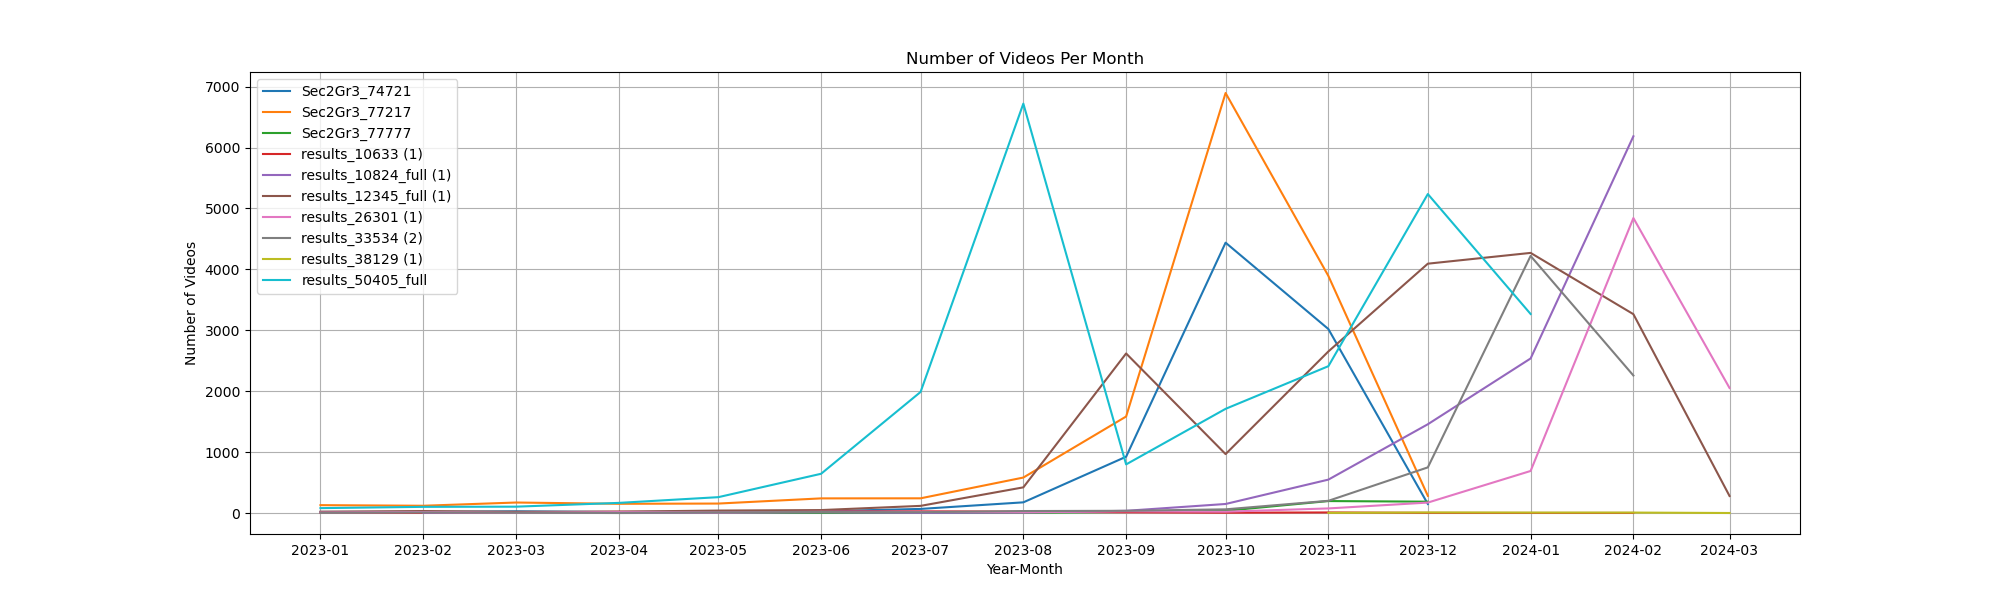
\includegraphics[width=\linewidth]{timeseries.png}
  \caption{Line chart showing user activity from January 2023 - March 2024. The X-axis values are the months. The Y-axis values are the number of videos watched. 
  \label{fig:timeseries}}
  \Description{User Activity.}
\end{figure}

There were 35671 unique post creators and 52632 unique video IDs across all users. We checked for overlaps in the videos the users watched (Figure 2). Overlaps were not common among all users but when there, they were in the hundreds of videos. For example, user 3 and user 7 had 775 similar videos watched, and user 8 and user 9 had 456.

\begin{figure}[ht]
  \centering
  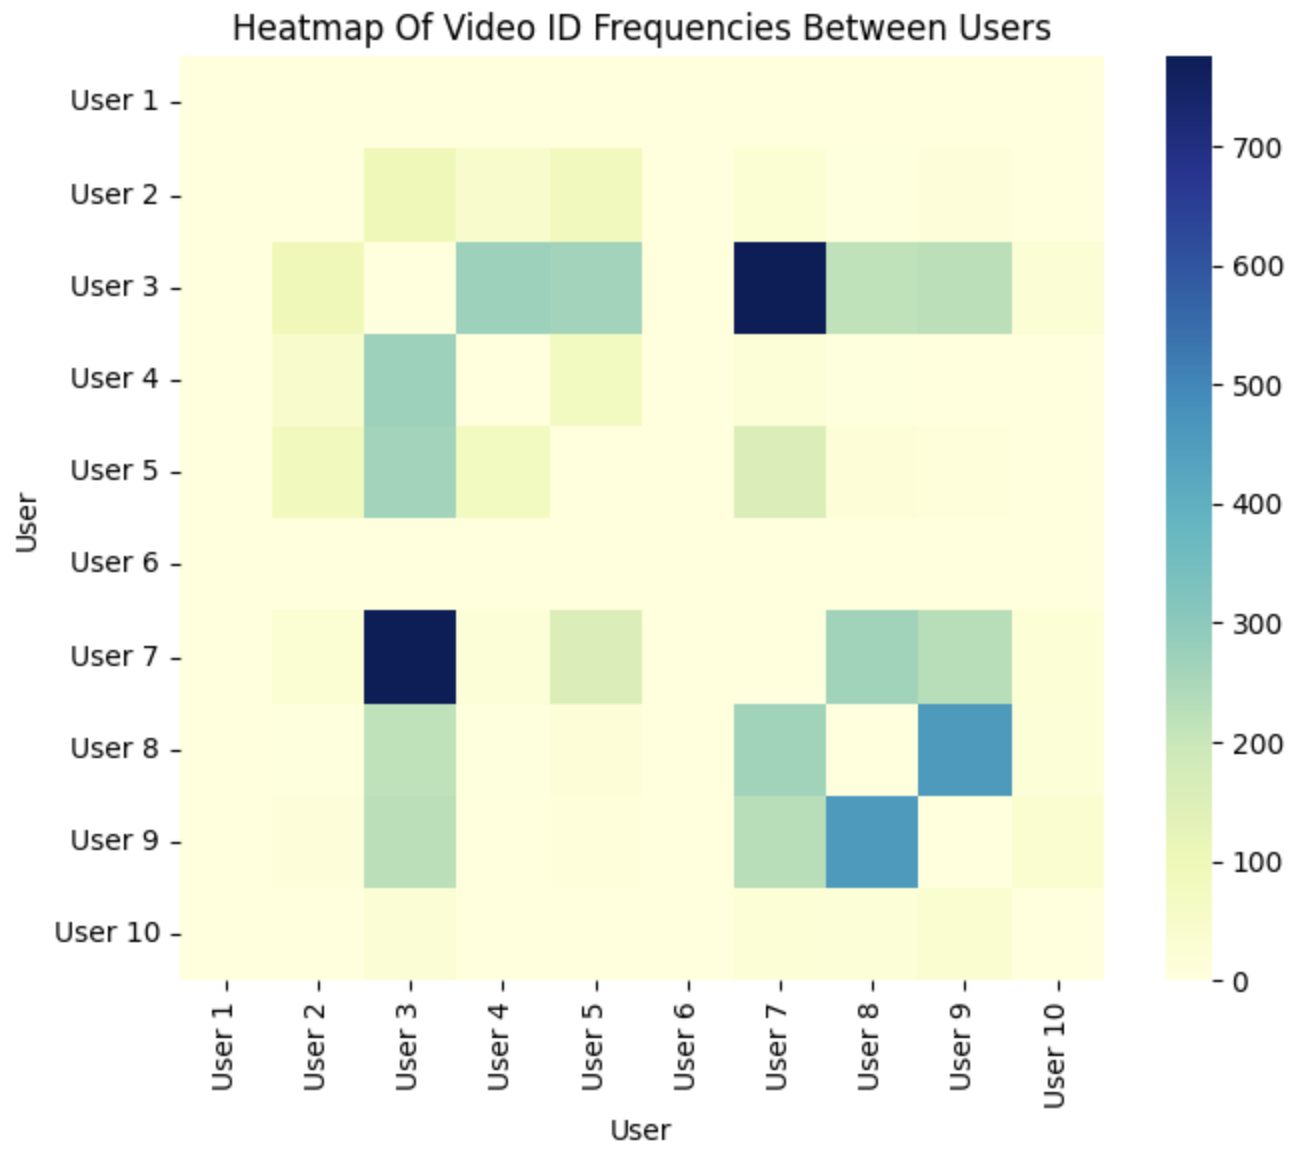
\includegraphics[width=\linewidth]{Video Overlaps.png}
  \caption{Heat map showing the number of video overlaps across all users. The X-axis and Y-values are the different users. 
  \label{fig:user-user}}
  \Description{Heat map of Video ID Frequencies Between Users.}
\end{figure}

\subsection{Methods}
\subsubsection{Experimental Setup}
For each csv file, we extracted all video descriptions and suggested words into a JSON file, the text corpus, resulting in 10 documents. depending on the analysis being performed, we either merged the documents into one file or analyzed the individual document. For both cases, we dropped all hash symbols and a majority of emojis for better model functionality. Before performing any analysis, we removed popular phrases such as 'fyp', 'trending', 'foryou', and 'viral' that may skew our results.

The hashtags data for all the users was converted into a JSON format for compatibility with the Universal Sentence Encoder (USE). The USE version 4 was utilized to generate embeddings for the TikTok hashtags. This pre-trained model, available through TensorFlow Hub, transforms text data into dense vector representations suitable for machine learning tasks.

\subsubsection{Data Analysis}
To analyze the results of our research on whether Wellesley students view similar content on TikTok, we utilized 4 methods:

First, we leveraged tf-idf to explore the dominant words for each user’s video content. We converted our data into a document-term matrix to obtain the keywords in each document that the model would use to predict the topics. We obtained the top 10 important words and their frequencies in the documents for each user while accounting for their universality across all users.

Secondly, we performed topic modeling on individual documents and the merged document to understand how spread the tiktok content is. We converted our data into a document-term matrix to obtain the keywords in each document that the model would use to predict the topics. Thereafter, we fit the Latent Dirichlet Allocation (LDA) model which grouped the words in the document-term matrix into topics. The model generated a topic-term matrix that associates each topic with 30 words. We set the number of topics to 5 for individual documents and 15 for the merged document. To generate the documents based on the topics, we transformed our document-term matrix into a document-topic matrix. 

Following the generation of embeddings, we used KMeans clustering to group similar hashtags based on similarity. The number of clusters was set to `k=5` as the best model indicated, and scikit-learn's implementation of KMeans was utilized for the clustering task. The resulting clusters were interpreted by examining the hashtags belonging to each cluster. This process allowed for understanding the common themes or topics represented by the hashtags within each cluster.

Finally, the T-SNE visualization generated fro the embeddings was overcrowded so, to further analyze the structure of the hashtag data, Principal Component Analysis (PCA) was performed to reduce the dimensionality of the data. The dimensionality was reduced to two principal components for visualization purposes.

Following PCA, KMeans clustering was applied again to the PCA-transformed data to obtain clusters. The clusters were visualized in a scatter plot, with each cluster represented by a distinct color. This visualization method facilitated the exploration of relationships between different hashtags and clusters.

\section{Results}
\subsection{Tf-IDF}
(Was to be edited by Rachel)

When we are looking at the important words for each user, we found a common interest in college, food, and Taylor Swift-related content - “college”,  “food”, and “taylor” exist in nine out of ten users’ top 10 TF-IDF score words. In addition, we find a widespread interest in traditionally defined female field content. For example, users 2, 3, 4, 5, 8, and 9 have “makeup”, while users 3, 4, 5, 7, 8, and 9 have “hair”. This result is expected since Wellesley College students is a historically all-women institution, so there is a shared interest in college life and content directed to women. Also, Taylor Swift is popular among the student body and popular on TikTok. However, we fail to find words that indicate a user’s particular interest, which deviates from the general trend across all users.

\begin{figure}[ht]
  \centering
  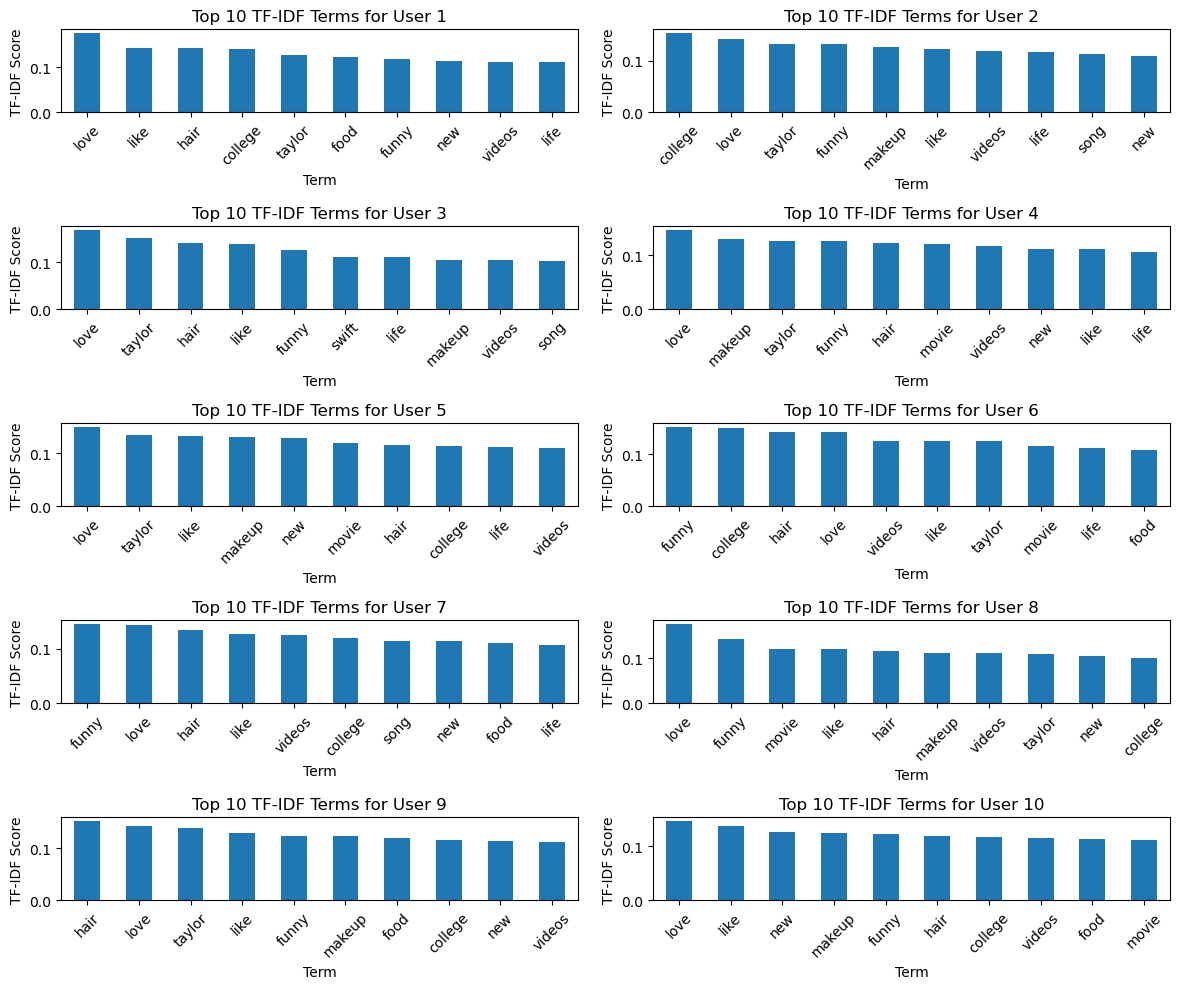
\includegraphics[width=\linewidth]{TFIDFold.png}
  \caption{Bar charts showing the most important words for all ten users. The X-axis values are the words. The Y-axis values are the tf-idf scores. 
  \label{fig:tf-idf}}
  \Description{Bar Charts of Top10 Tf-IDF Terms For All Users.}
\end{figure}

At this early stage of our analysis, common hashtags “foryou”, “tiktok”, and “like” still have high TF-IDF scores even if they appear in most users' documents and cannot indicate users' specific content interests. Also, there are over 40k columns, each representing one unique word and showing the TF-IDF score of each user for that word. These two problems show that some words appear for most of the user's documents, and some document words may be misspelled and thus only occur once, but still are on one column. To restrict the words used in calculating TF-IDF scores, we set the maximum occurrence threshold for an "important word" to 70\% of the users' documents and excluded all words that appeared only once. In addition, users 1, 6, and 10 all have less than 1k content viewing history, so we exclude them from our analysis. After this process, the number of columns decreases to 23453, but is still a large data frame.

Now, the TF-IDF score tells us more about each user's particular interest. For example, user 2 is interested in American pop culture and music, "Khia" is a famous American rapper, "Kartel" is a digital creative label, and "Bibbidi" is the song in Cinderella and recently in trend to film funny videos. User 5 is more interested in vacation destinations, ice hockey, and Korean rap culture - "Samoa" is a Polynesian island country famous for its beaches and natural scenery, "DeSantis" can stand for Ronald Dion DeSantis, the governor of Florida, who pushes new policies like closing the beaches early that are related to Miami vacation, "Monahan" stands for Sean Monahan, a Canadian ice hockey center. Although some of the important words are less conclusive of the interest they indicate, for example, "Duvall" for user 5, which can be a misspelling of Duval, a county in Florida and aligns with our hypothesis that users are interested in vacation in Florida, this TF-IDF analysis gives us a general sense of each user's interest.


\begin{figure}[ht]
  \centering
  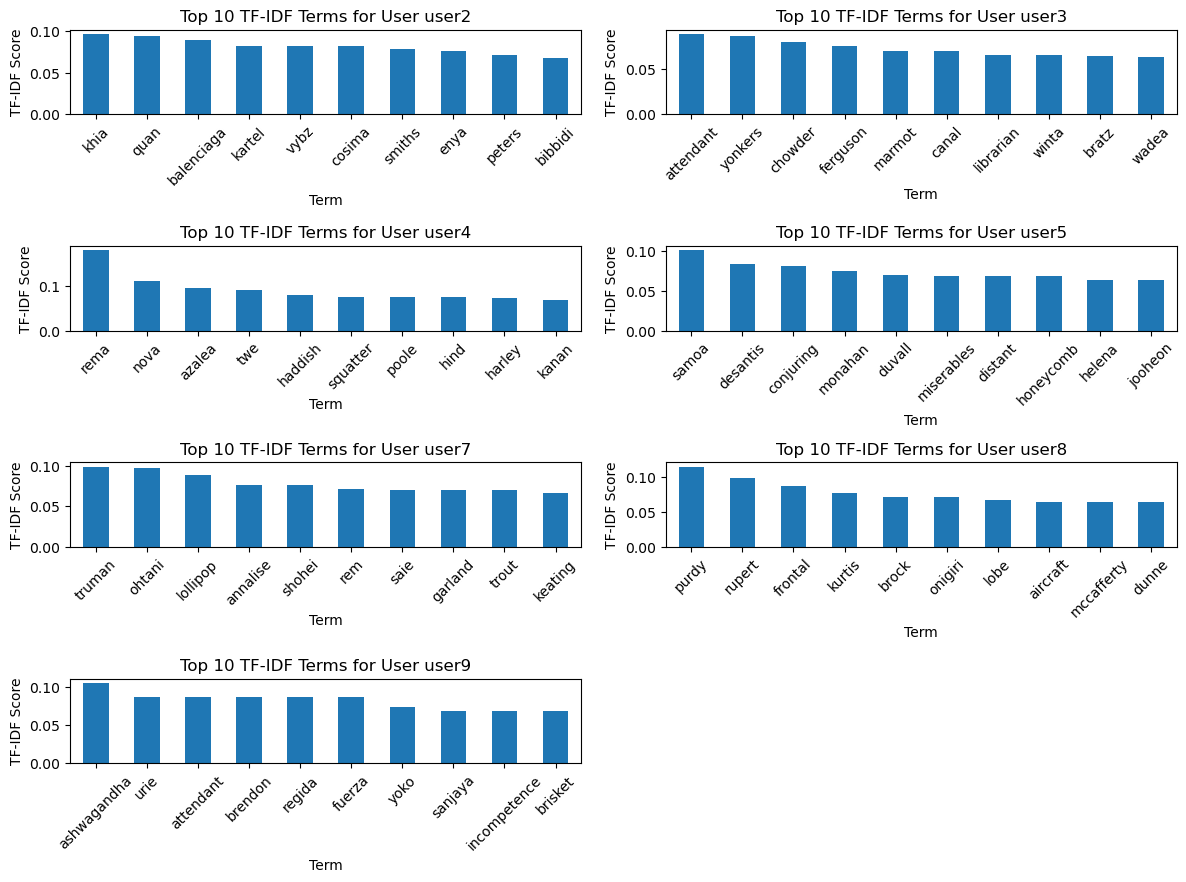
\includegraphics[width=\linewidth]{tfidf.png}
  \caption{Bar charts showing the most important words for seven users (excluding users with less than 1000 video viewing history). The X-axis values are the words. The Y-axis values are the tf-idf scores. 
  \label{fig:tf-idf}}
  \Description{Bar Charts of Top10 Tf-IDF Terms Excluding Unregular Users.}
\end{figure}

\subsection{Topic Modeling}
In our investigation into the variability of content consumption among students at Wellesley College, our topic modeling analysis yielded heterogeneous findings. The topics generated exhibited a varied range of how well words in topics fit together, with some displaying a high degree of semantic similarity while others appeared disjointed. For instance, Topic 2 displayed a notable cohesion around the subject of food (Table 2). Similarly, Topic 8 predominantly comprised terms associated with celebrities and popular culture, although 'acne' was also strangely linked to this theme. Conversely, Topics 5 and 10 contained terms that exhibited minimal thematic coherence.

\begin{table*}[ht]
  \caption{All Users Topic-term distribution}
  \label{tab:context}
  \begin{tabular}{cl}
    \toprule
     Topic & Terms\\
    \midrule
    \texttt 0 & makeup Christmas skin beauty grwm day skincare tutorial tree gift,\\
    \texttt & face foundation make michael eye products blush look sabrina routine,\\
    \texttt & carpenter card haul sephora concealer victoria ready chipotle san care. \\    
    \texttt 1 & new nyc york apartment mom interview history life dating work, \\
    \texttt & city link bio park south questions corporate job lana relationship, \\
    \texttt & mexico john time got coquette street subway funny year living. \\
    \texttt 2 & recipe food chicken recipes cheese girls birthday mean make free, \\
    \texttt & dinner cake cooking rice cup pasta cream ideas add meal, \\
    \texttt & oil easy making thanksgiving milk chocolate pepper bell salad butter. \\
    \texttt 3 & hair disney water girl black white soup mascara brown game, \\
    \texttt & cut haircut crochet blue brush color accent stanley fnaf hairstyles, \\
    \texttt & teeth curly glass mexican twilight hairstyle cup bangs lunch tutorial. \\
    \texttt 4 & lip funny olivia cleaning bachelor rodrigo williams doctorwho snl wendy, \\
    \texttt & prank joey love comedy family trump moments davidtennant balm shoes, \\
    \texttt & videos edit perfume lips clean shane summer emma gloss maria. \\
    \texttt 5 & avatar dance home parents candy smith nails princess mac apple airbender, \\
    \texttt & iphone rachel zuko proposal bathroom podcast marriage tea live girl action, \\
    \texttt & cookie alex nail bear dancing kitchen kids board. \\
    \texttt 6 & college school student doctor life university taylorswift ice dad david tennant, \\
    \texttt & money swifttok science football swiftie medical major high tiktok musical, \\
    \texttt & law students singing harvard basketball theatre song engineering med. \\
    \texttt 7 & like just know think good little love don dont time people dune way life, \\
    \texttt & replying sister year did feel let want really brother say big right hard look, \\
    \texttt & family got. \\
    \texttt 8 & taylor swift stitch song music super songs golden tour travis bowl austin, \\
    \texttt & eras kelce usher grammys hamilton love justin lyrics concert globes acne, \\
    \texttt & guitar jennifer black jacob beyonce singing bella. \\
    \texttt 9 & food dress outfits outfit tiktok teacher couple fashion room couples ideas, \\
    \texttt & target african clothes videos spanish language dresses ootd fall life, \\
    \texttt & style french pregnant speaking orange sydney hamster english clothing. \\
    \texttt 10 & book joe things books replying starbucks korean booktok pizza noah kim, \\
    \texttt & greenscreen indian mitski miami therapy song tiktok trader tattoo kpop, \\
    \texttt & bts, poetry poor pants saltburn guess roommate scott graduation. \\
    \texttt 11 & cat baby wedding videos cats tiktok games cute funny barbie hunger, \\
    \texttt & date snow art jeans animals josh tom pet zendaya painting drake edit, \\
    \texttt & twins animal gray kittens catsoftiktok lucy old. \\
    \texttt 12 & movie car house harry travel scene timothee beyonce body long love, \\
    \texttt & movies chalamet potter kylie time chicago shop film wonka fish tiktok, \\
    \texttt & wig ending sza scary ocean family horror garden. \\
    \texttt 13 & love boston halloween costume jackson thrift nicki blind percy minaj, \\
    \texttt & ariana megan thrifting grande anime ring haul spongebob stallion kpop, \\
    \texttt & thee gym fortnite gojo store finds massachusetts sarah elementary empire. \\
    \texttt 14 & dog filter bag dogs coffee face tiktok office green eyes business lee tote, \\
    \texttt & videos deodorant puppy effect funny grey anatomy cake test black, \\
    \texttt & bags google keith shop phone coach dogsoftiktok. \\
    \bottomrule
  \end{tabular}
\end{table*}
Upon examination of the bar chart (Figure 5) illustrating the distribution of video descriptions and suggested terms for each topic across all users, Topic 7 emerged as the predominant theme, vaguely centered around relationships, constituting 17\% of the total distribution while each of the other topics constituted less than 10\%.

\begin{figure}[ht]
  \centering
  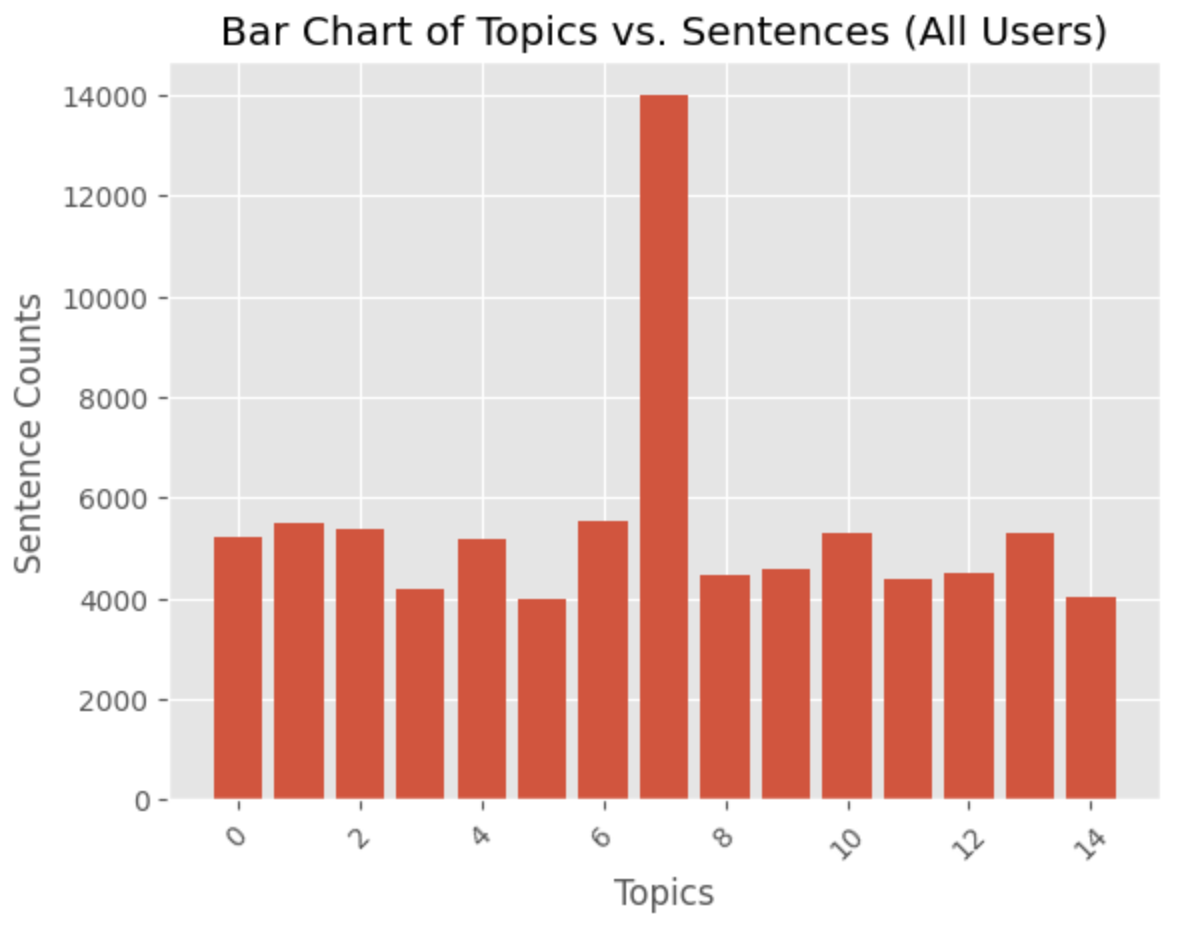
\includegraphics[width=\linewidth]{General Topic Distribution.png}
  \caption{Bar chart showing the counts of video descriptions and suggested words for each topic across all users. The X-axis values are the topics. The Y-axis values are the total counts. 
  \label{fig:topic counts}}
  \Description{Bar Chart of Topic Counts.}
\end{figure}
To ascertain the presence and magnitude of any thematic overlaps, we constructed a heat map (Figure 6) depicting the probabilities of topic occurrence for each user and vice versa. Following Topic 7, Topic 6, characterized as student life, emerged as the next most prevalent among users.

\begin{figure}[ht]
  \centering
  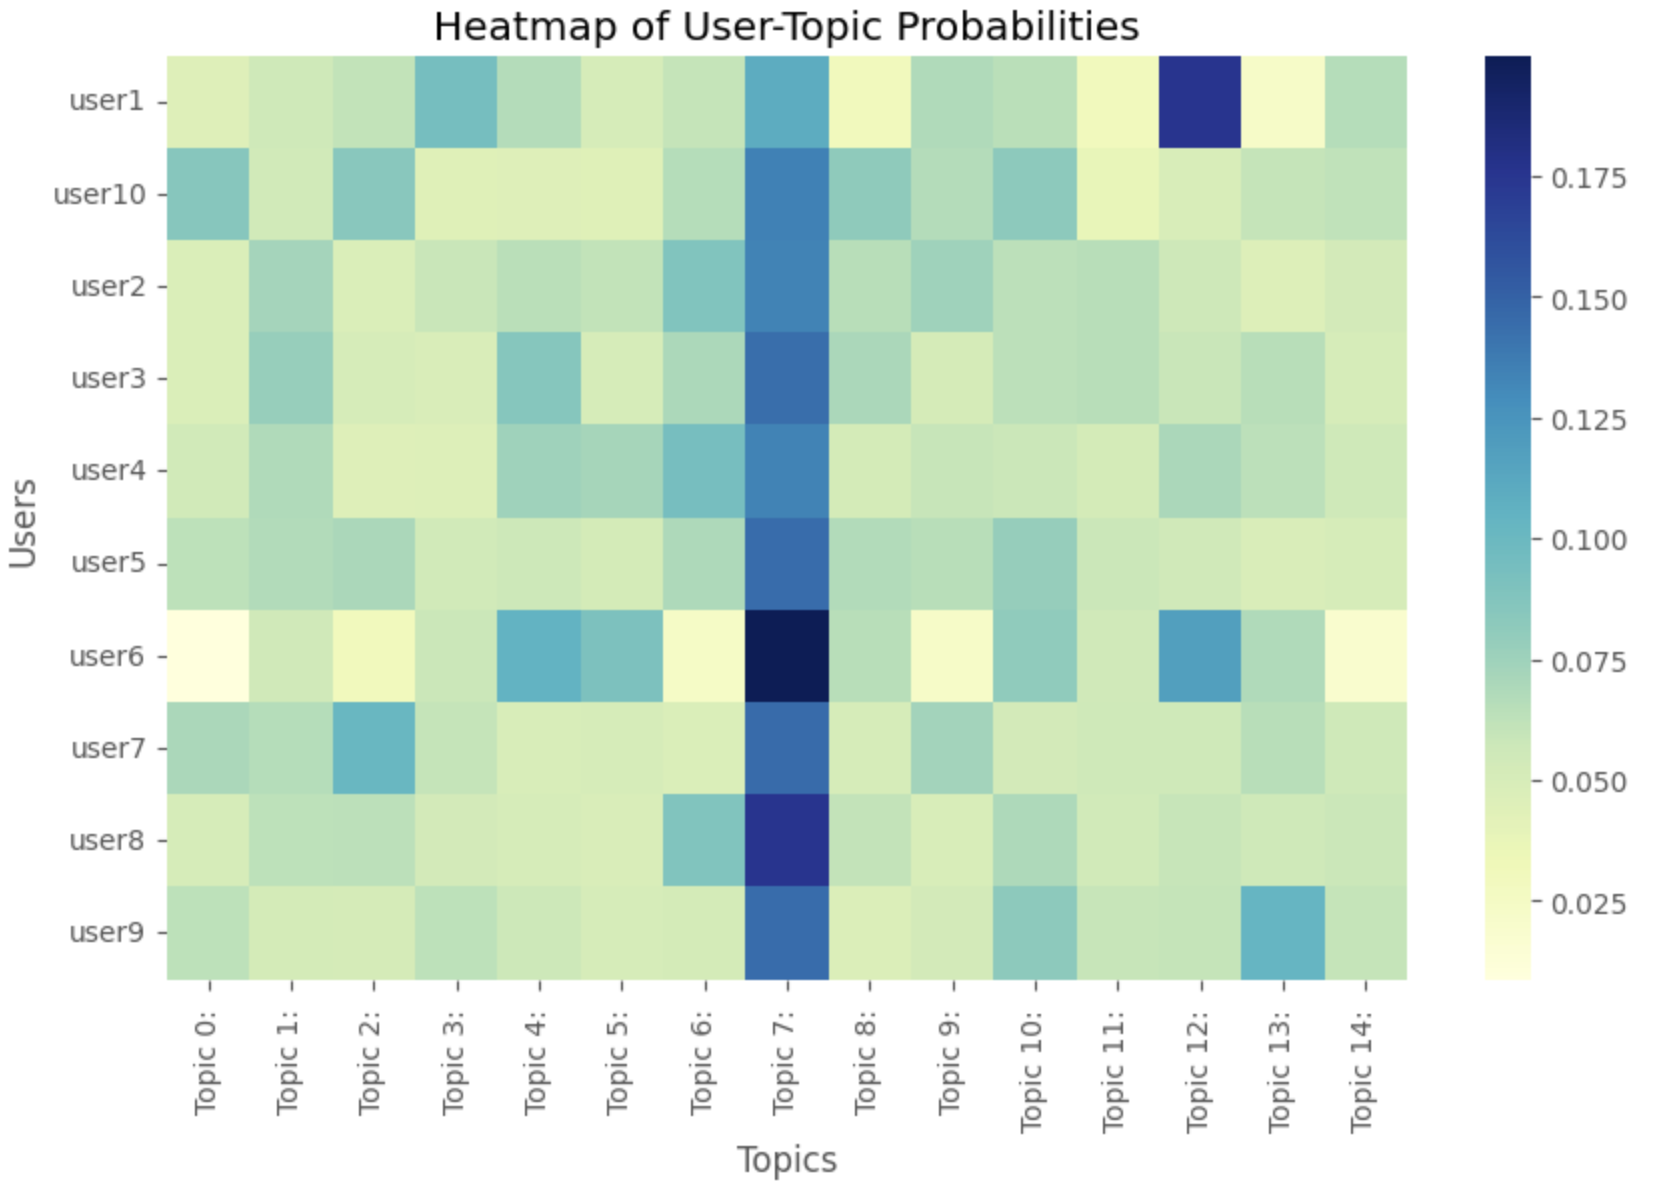
\includegraphics[width=\linewidth]{User-Topic.png}
  \caption{Heat map showing the average probabilities of all the topics across all users. The X-axis values are the topics. The Y-axis values are the different users. 
  \label{fig:user-topic}}
  \Description{Heat map of User-Top Probabilities.}
\end{figure}

To corroborate the topics for each user displayed on the heatmap, we summarized the dominant topics for each user in Table 3.

\begin{table*}[ht]
  \caption{Topic-term distribution}
  \label{tab:context}
  \begin{tabular}{lcl}
    \toprule
     User & Dominant Topic & Terms\\
    \midrule
    \texttt user1 & 3 & bible showers food truth reads amazon cooking night jesus bed life,\\
    \texttt & & amazonfinds videos cold showering buy choi zach tiktokmademebuyit fav,\\
    \texttt & & things christian day tiktok products god cleaning black bibles pink. \\    
    \texttt user2 & 0 & ghanatiktok teacher funny song parents mom africantiktok nicki tiktok, \\
    \texttt &&  nigeriantiktok rap minaj makeup life videos comedy lay viralvideo kai jersey, \\
    \texttt && ghanafuodotcom like music nigeria freestyle ghana dance bag concert cat. \\
    \texttt user3 & 0 & college love girls funny mean movie hair disney mom life just, \\
    \texttt && taylorswift olivia song snl williams tiktok rodrigo moments black, \\
    \texttt && makeup dad car world girl couple people student avatar broadway. \\
    \texttt user4 & 4 & college dune student university makeup movie hair life tiktok boston wendy, \\
    \texttt && girl teacher timothee science chalamet computer austin spanish maya, \\
    \texttt && twilight engineering major smith just bag people butler make school. \\
    \texttt user5 & 1 & love like baby austin nyc mcbroom coffee trend couple bachelor, \\
    \texttt && new joey just tiktok song date dance night girl guy time, \\
    \texttt && pizza bell people starbucks know podcast taco life cleaning. \\
    \texttt user6 & 3 & hakari chel euphoria charger car husband dorado road maddy zoe, \\
    \texttt && jjk cat ebarb rich married disney edits cosplay kashimo nate, \\
    \texttt && retractable shop mia dio getting dating kitten bell myer tulio. \\
    \texttt user7 & 1 & taylor love new filter swift cheese replying taylorswift tour nyc eras, \\
    \texttt && jeans skin sabrina song cottage girl carpenter foundation like year, \\
    \texttt && funny sunscreen stanley body free disney birthday color york. \\
    \texttt user8 & 0 & college hair friends student palestine life study tiktok home love, \\
    \texttt && funny dog university empire food way roman girls say like work, \\
    \texttt && people pretty know friend travel little disney think day. \\
    \texttt user9 & 2 & hair love jjk gojo filter girl replying edit know jujutsukaisen new, \\
    \texttt && anime funny eyes art life choso cut jujutsu haircut blue, \\
    \texttt && zendaya think movie nanami got kaisen time dance song. \\
    \texttt user10 & 3 & sydney sweeney maybelline thanksgiving little woman christmas food, \\
    \texttt && game play let language sat song hello skibidi wonyoung trap kindle tea, \\
    \texttt && kpop sunwoo tibet angels celeb video concert coffee smith service. \\
    \bottomrule
  \end{tabular}
\end{table*}

\subsection{K Clustering }
The dispersion of the hashtags within each cluster as indicated by Figure 7 highlights the diversity and commonality in content preferences among users. 

\begin{figure}[ht]
  \centering
  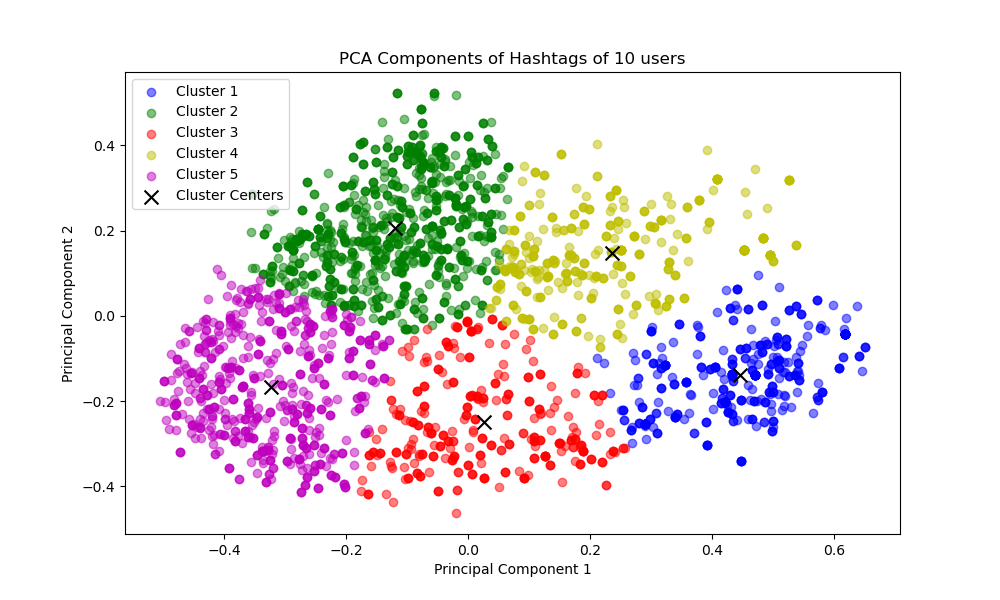
\includegraphics[width=\linewidth]{PCA.png} 
  \caption{t-SNE visualization of the Hashtag clusters after dimensionality reduction was done. The X-axis represents the 1st principal component analysis. The Y-axis represents the 2nd principal component analysis.}
  \label{PCA Visualization of Hashtags with Clusters.}
  \Description{ t-SNE visualization of the Hashtag Clusters.}
\end{figure}

Firstly, the dispersion within each cluster, as indicated by the spread of data points along principal components (PC1 and PC2), reveals the variability in content preferences among users within the same cluster (Figure 7). For instance, Cluster 1 exhibits a relatively lower spread, suggesting a higher degree of consensus in the type of content consumed among its members. Conversely, Clusters 4 and 5 display wider spreads, indicating diverse content preferences and interests among users within these clusters. This dispersion within clusters suggests that while some groups may have more homogeneous content consumption habits, others show greater diversity in their interests. 

On the other hand, the relationships between clusters, observed through their spatial arrangement in the PCA-transformed space, provide insights into the similarities and differences in content consumption across different user groups. The proximity of clusters to each other indicates similarities in the types of content consumed by users across these groups. For example, Cluster 4 overlaps with Clusters 1, 2, and 3, which suggests that despite their distinct cluster assignments, users within these clusters consume similar types of content. Contrarily, clusters that are farther apart in the PCA plot represent user groups with more distinct content preferences. This suggests that while there may be common trends, students also exhibit individual preferences and interests in the content they consume on TikTok.

Examining the contents of each cluster provides further insight into the themes captured by the hashtags. Cluster 1, depicted in its word cloud (Figure 8), prominently features references to Taylor Swift, suggesting a focus on the artist's content or related topics.

In Cluster 2 (Figure 9), the word cloud reveals a medley of pop culture, movie references, and celebrity gossip, indicating a broad interest in entertainment and celebrity news among users.

Health-related topics dominate Cluster 3 (Figure 10), with mentions of Taylor Swift alongside health-related terms, potentially indicating wellness topics. Cluster 4 (Figure 11), revolves around "booktok" and zodiac signs, but also contains random words such as “private chef”.

Cluster 5 (Figure 12), though sparse in terms of words, centers around discussions related to the latest movie of the Hunger Games franchise, providing a glimpse into ongoing conversations about this particular film.

The diverse array of words within each cluster, as depicted in the word clouds, aligns with the observations derived from the PCA visualization.

\begin{figure}[ht]
  \centering
  \Description{Word Clouds to show the words in each cluster}
  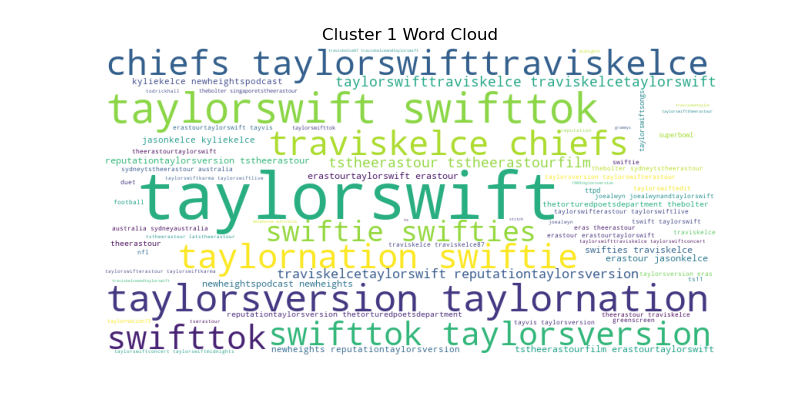
\includegraphics[width=0.8\linewidth]{cluster_1_wordcloud.png} 
  \caption{Word Cloud showing words that make up cluster 1}
  \label{fig:WordsInCluster1}
  \end{figure}

\begin{figure}[ht]
  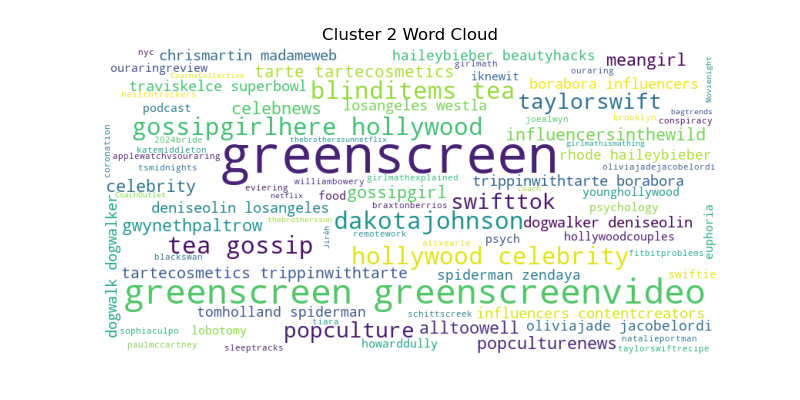
\includegraphics[width=0.8\linewidth]{cluster_2_wordcloud.png} 
  \caption{Word Cloud showing words that make up cluster 2}
  \label{fig:WordsInCluster2}
\end{figure}

\begin{figure}[ht]
  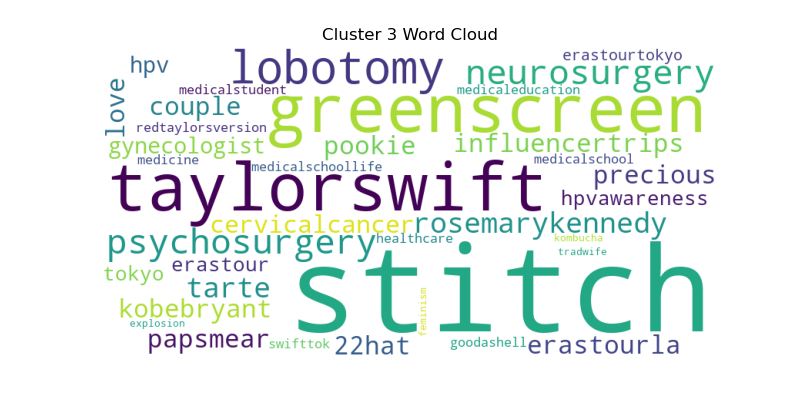
\includegraphics[width=0.8\linewidth]{cluster_3_wordcloud.png} 
  \caption{Word Cloud showing words that make up cluster 3}
  \label{fig:WordsInCluster3}
\end{figure}

\begin{figure}[ht]
  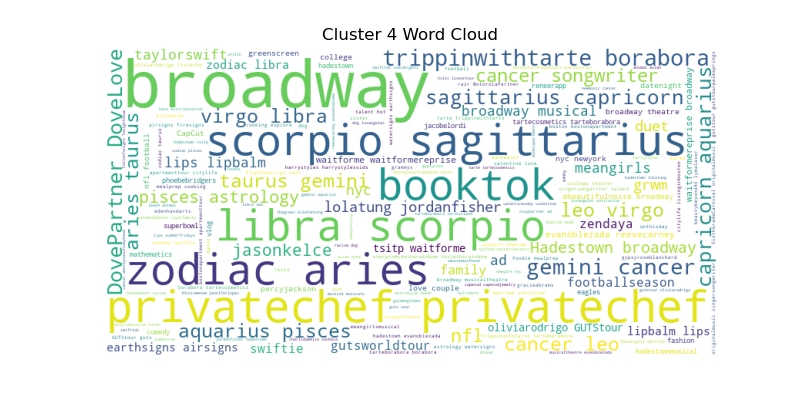
\includegraphics[width=0.8\linewidth]{cluster_4_wordcloud.png} 
  \caption{Word Cloud showing words that make up cluster 4}
  \label{fig:WordsInCluster4}
\end{figure}

\begin{figure}[ht]
  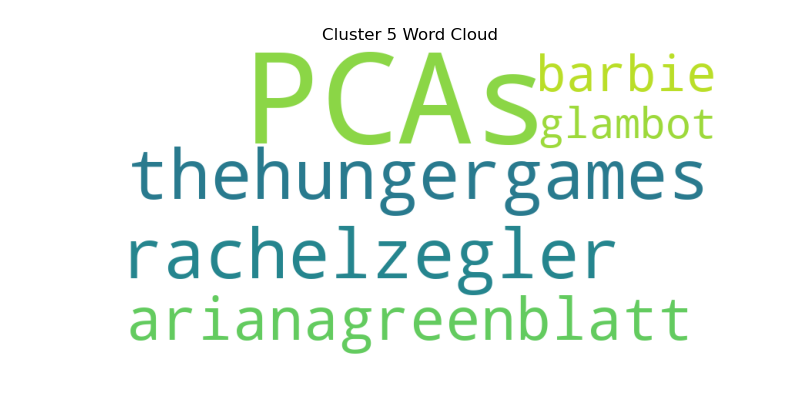
\includegraphics[width=0.8\linewidth]{cluster_5_wordcloud.png} 
  \caption{Word Cloud showing words that make up cluster 5}
  \label{fig:WordsInCluster5}
\end{figure}

\section{Conclusion}
\subsection{Discussion}
Our results indicate a mix of shared trends and individual preferences among Wellesley College students. From the methods utilized, we see a degree of consensus in content consumption with large interests in pop culture \& celebrities - evidenced by terms such as 'Taylor Swift', 'Olivia Rodrigo', 'celebnews', the 'Grammys', 'kpop', 'booktok'-, food \& cooking - seen through 'recipe', 'oil' 'chicken', and 'thanksgiving' -, skin care \& beauty - evidenced by phrases such as 'makeup', 'foundation', and 'sephora' -, and college-related content. These findings show that Wellesley College students view similar content on TikTok and have overlapping themes.

Beyond these shared themes, individual preferences are also significant influencers of content consumption habits among Wellesley students on TikTok. For instance, while there are common interests observed across the user documents, distinct preferences surface within specific users. Notably, unique dominant themes among individual users include religion (user1), culture (user2), academia (user4), and pop culture (user7) (Table 3). While shared trends exist, students' unique interests and backgrounds shape their experiences on the platform.

\subsection{Limitations}
The primary challenge encountered during data analysis stemmed from inconsistencies in the timestamps of users' browsing history. For example, while some users had data spanning only the year 2023, others had data solely from 2024, reflecting differences in their time of joining TikTok and their activity on the platform. Without consistent timestamps, conducting accurate temporal analyses, such as identifying trends or patterns over time, became challenging. 

While our study provides valuable insights into the content consumption habits of Wellesley students, it does not explore external factors such as cultural influences or individual motivations unique to Wellesley College students. These external factors could significantly shape students' content preferences and engagement on TikTok. By excluding these elements, our research provides a somewhat incomplete picture of the relationship between personal motivations, cultural influences, and content consumption behaviors.

Our conclusions rely on previous literature that cites a correlation between user interest, and TikTok suggested content. There is an assumption that user interests shape users' content feeds. But, the inverse is possible. TikTok's suggested content may influence, and inflate users' interests. TikTok's proprietary algorithms may distort our results. It is unclear whether trends among Wellesley College students' viewership and engagement are representative of their interests outside of TikTok.  

\subsection{Future Work}
For future investigations, one could obtain data with fewer timestamp discrepancies and establish a standardized framework for timestamp synchronization. This could significantly improve the reliability of temporal analyses and allow for a comparative analysis of similarity over time. 

Analyzing data for users before and after they arrive at Wellesley to discern any shifts in their TikTok usage patterns would provide valuable insights into the evolving dynamics of their content consumption habits. 

Related studies could examine the impact of TikTok usage on academic performance and social interactions among Wellesley College students. This could provide valuable insights into the broader implications of social media usage within educational settings. Addressing these areas in future research endeavors would deepen our understanding of TikTok usage among Wellesley College students.

\printbibliography %Prints bibliography

\end{document}
\endinput